	\documentclass[twoside]{article}
\usepackage{../../estilo-ejercicios}
\renewcommand{\baselinestretch}{1,3}
%--------------------------------------------------------
\begin{document}

\title{Ejercicios de Topología Algebraica}
\author{Javier Aguilar Martín}
\maketitle

\begin{ejercicio}{3.2.1}
Suponiendo conocida la estructura del cup producto en el toro $S^1×S^1$, calcular la estructura de cup producto en $H^*(M_g)$ para $M_g$ la superficie cerrada orientable de género $g$ usando la apliación cociente de $M_g$ a la suma puntual de $g$ toros, mostrada debajo.


\begin{figure}[h!]
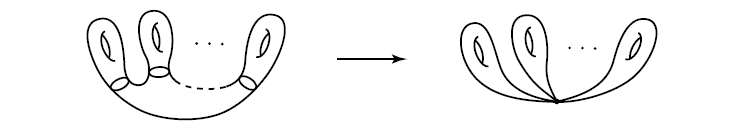
\includegraphics[scale=0.6]{mg}
\end{figure}
\end{ejercicio}
\begin{solucion}
%\url{https://agmablog.files.wordpress.com/2014/08/topology-2-hmwk-2.pdf}
%\url{http://web.math.ku.dk/~moller/f03/algtop/opg/S3.2.pdf}
%\url{http://math.stanford.edu/~ralph/math215c/solution2.pdf}
%\url{http://math.ucr.edu/~res/math205B-2012/helpfile.pdf}

Tenemos 
\[
H_n(M_g)=\begin{cases}
\Z & n=2\\
\Z\underbrace{\oplus\cdots\oplus}_{2g}\Z & n=1\\
\Z & n=0\\
0 & c.c.
\end{cases}
\]
por lo que del teorema de coeficientes univerales deducimos que el cup producto $H^q(M_g)\times H^l(M_g)\to H^{q+l}(M_g)$ es trivial en todos los casos salvo $q=l=1$ (si $ql=0$, entonces es simplemente producto por escalares). Tenemos también por el teorema de coeficientes universales que $H^1(M_g)=\Z^{2g}$ y $H^2(M_g)=\Z$. Por otro lado, la aplicación cociente $q:M_g\to\bigvee_{i=1}^g M_1$ induce una homomorfismo de anillos graduados $q^*:H^*(\bigvee_{i=1}^g M_1)\to H^*(M_g)$. Tenemos además el isomorfismo $\widetilde{H}^*(\bigvee_{i=1}^g M_1)\cong\bigoplus_{i=1}^g \widetilde{H}^*(M_1)$. 

Por el cálculo del cup producto en $M_1$, para todo $i=1,\dots, g$, sabemos que podemos tomar generadores $\alpha_i$ y $\beta_i$ de $H^1(M_1)$ correspondientes a la $i$-ésima copia de $M_1$ en la suma puntual cumpliendo $h(\alpha)=[a_i]^*$ y $h(\beta)=[b_i]^*$ (dual de los generadores de $H_1(M_1)$) de modo que si $\gamma_i$ es un generador de $H^2(M_1)$ correspondiente a esa misma copia de $M_1$ (cumpliendo $h(\gamma)=[c_i]^*$, con $[c_i]$ generador de $H_2(M_1)$), entonces $\alpha_i\smile \beta_i=\gamma_i$ y $\alpha_i\smile \alpha_i=\beta_i\smile \beta_i=0$. 

Si $c_i$ representa un generador de $H_2(\bigvee_{i=1}^g M_1)$ y $C$ representa un generador de $H_2(M_g)$, entonces, como se puede observar geométricamente, la aplicación cociente induce a nivel de cadenas la aplicación $C\mapsto c_1+\cdots+c_1$, por lo que en las cocadenas se induce las aplicaciones $c_i^*\mapsto C^*$ para todo $i$. 

Similarmente, si $A_i,B_i$ representan generadores de $H_1(M_g)$ y $a_i,b_i$ representan generadores de $H_1(\bigvee_{i=1}^g M_1)$, el cociente induce a nivel de cadenas la aplicación $A_i\mapsto a_i$, $B_i\mapsto a_i$, de modo que en cocadenas obtenemos $a_i^*\mapsto A_i^*$, $b_i^*\mapsto B_i^*$. 

Finalmente, la naturalidad del cup producto nos da el diagrama conmutativo
\[
\begin{tikzcd}
H^1(\bigvee_{i=1}^g M_1)\times H^1(\bigvee_{i=1}^g M_1) \arrow[r, "\smile"] \arrow[d, "q^*"'] & H^2(\bigvee_{i=1}^gM_1) \arrow[d, "q^*"] \\
H^1(M_g)\times H^1(M_g) \arrow[r, "\smile"] & H^2(M_g)
\end{tikzcd}
\]
con lo que $[A_i^*]\smile [B_i^*]=[C^*]$, $[A_i^*]\smile [A_i^*]=[B_i^*]\smile [B_i^*]=0$. También obtenemos por la conmutatividad y por la estructura del producto de anillos (recordemos que la fila superior se reescribe en términos de productos) que $[A_i^*]\smile [A_j^*]=[B_i^*]\smile [B_j^*]=[A_i^*]\smile [B_j^*]=0$ para $i\neq j$. Con todo, tenemos determinado el cup producto que buscábamos, ya que por el teorema de coeficientes universales y el hecho de que los grupos de homología de $M_g$ son libres y finitamente generados, $h$ es un isomorfismo y los que hemos dado son todos los generadores. 



%NO ESTOY SEGURO DE ESTO QUE ESTOY DICIENDO A CONTINUACIÓN, PENSARLO Y SI NO PREGUNTARLO U OMITIRLO
%
%En concreto, hemos encontrado que la estructura que tiene es la de un cociente del álgebra exterior $\bigwedge_{\Z}[A_1^*,\dots, A_g^*,B_1^*,\dots, B_g^*]$ surgido al cocientar por el ideal generado por las expresiones que hemos visto que se anulan, esto es, $\{A_i^*\smile A_j^*,B_i^*\smile B_j^*,A_i^*\smile B_j^*\mid i\neq j\}$.
\end{solucion}

\newpage

\begin{ejercicio}{3.2.9}
Probar que si $H_n(X; \Z)$ es libre para todo $n$, entonces $H^*(X; \Z_p)$ y $H^*(X; \Z)\otimes \Z_p$ son isomorfos como anillos, por lo que en particular la estructura de anillo con coeficientes en $\Z$ determina la estructura de anillo con coeficientes en $\Z_p$. 

\end{ejercicio}
\begin{solucion}
%\url{https://www2.math.ethz.ch/education/bachelor/lectures/fs2014/math/alg_topo/sol3.pdf}

Como no se indica sobre qué anillo se hace el producto tensorial, sobreentendemos que es sobre $\Z$. Por el teorema de coeficientes universales y por ser $H_n(X;\Z)$ libre para todo $n$ tenemos que $h_{\Z}:H^n(X;\Z)\to\Hom(H_n(X;\Z),\Z)=\prod_{i\in I_n}\Z$ y $h_{\Z_p}:H^n(X;\Z_p)\to\Hom(H_n(X;\Z),\Z_p)=\prod_{i\in I_n}\Z_p$ son isomorfismos de grupos, donde $I_n$ es el conjunto de índices que recorren los generadores de $H_n(X;\Z)$. Las igualdades se tienen por la linearidad del functor $\Hom$ con respecto a la suma directa en la primera coordenada. Tenemos entonces $H^*(X;\Z)=\bigoplus_n(\prod_{i\in I_n}\Z)$ y $H^*(X;\Z_2)=\bigoplus_n(\prod_{i\in I_n}\Z_p)$.

La idea ahora es definir una aplicación bilineal y sobreyectiva $f:H^*(X;\Z)\times \Z_p\to H^*(X;\Z_p)$ que sea inyectiva y homomorfismo de anillos al definirla sobre el producto tensorial. Como el producto tensorial se distribuye sobre la suma directa basta definir para cada $n$ una aplicación $f_n:(\prod_{i\in I_n}\mathbb{Z})\times\mathbb{Z}_p\to \prod_{i\in I_n}\mathbb{Z}_p$ (además para que sea homomorfismo de anillos graduados necesitamos que $f$ respete los grados, de ahí el codominio). La definimos como $f_n(\prod_i a_i,b)=\prod_i [a_i] b$ (donde $[a_i]$ es la clase en $\Z_p$). La aplicación es claramente bilinear y sobreyectiva, por lo que induce un homomorfismo de grupos sobreyectivo al tomar producto tensorial. Veamos que es inyectiva en el producto tensorial. Supongamos que $f_n((\prod_ia_i)\otimes 1)=0$. Entonces $\prod_i[a_i]=0\in\prod_i\mathbb{Z}_p$, por lo que $[a_i]=0\in\mathbb{Z}_p$ para todo $i$, por lo que $a_i=pa_i'$. De este modo, 

$$\left(\prod_ia_i\right)\otimes 1=\left(\prod_i pa_i'\right)\otimes 1=p\left(\prod_ia_i'\right)\otimes 1=\left(\prod_ia_i'\right)\otimes p=\left(\prod_ia_i'\right)\otimes 0=0$$
Es fácil ver que los elementos de la forma $(\prod_ia_i)\otimes 1)$ generan $H^n(X;\Z)\otimes\Z_p$ como grupo, por lo que esto prueba la inyectividad. 

Con esto hemos probado $H^n(X;\Z)\otimes \Z_p\cong H^n(X;\Z_p)$ como grupos. Ahora bien, dado un cociclo  $\phi\in C^n(X)$ y $r\in \Z_p$, este isomorfismo identifica $[\phi]\otimes r\in H^n(X)\otimes \Z_p$ con la clase en $H^n(X;\Z_p)$ representada por el cociclo en $C^n(X;\Z_p)$ que toma una cadena $\sigma\in C_n(X)$ y la envía a $[\phi(\sigma)]r$. Es inmediato entonces que este isomorfismo respecta las estructuras de anillos.
%Definimos ahora una aplicación bilineal y sobreyectiva $f:(\prod_{i\in I}\mathbb{Z})\times\mathbb{Z}_p\to \prod_{i\in I}\mathbb{Z}_p$ que induzca un isomorfismo de grupos cuando se define sobre el producto tensoria.


%$H^n(X;R)\cong\Hom(H_n(X;\Z),R)\cong\Hom(H_n(X),\Z)\otimes R\cong H^n(X)\otimes R$ como grupos abelianos. EL ISOMORFISO QUE CAMBIA R POR Z Y PRODUCTO TENSORIAL LO TENGO QUE PENSAR (ALOMEJOR TIENE QUE VER CON LA ADJUNCIÓN HOM-TENSOR Y QUE HOM(Z,R)=R) CREO QUE NO VA A PODER SER SI LA HOMOLOGÍA NO ES FINITAMENTE GENERADA, ASÍ QUE PREGUNTAR SI ESTE CASO PARTICULAR VALE. EN ESTE CASO CREO QUE SI HAGO TENSOR DEL PRODUCTO CON ZP ME SALE PRECISAMENTE EL PRODUCTO DE ZP PERO ME TENGO QUE ASEGURAR (DE TODOS MODOS CREO QUE ESTO ES LO MISMO QUE TENGO HECHO EN LA PREGUNTA QUE HICE, ASÍ QUE BASTARÍA REINTERPRETAR ESE MORFISMO COMO LO QUE TENGO DEBAJO)


%
%For example, if I define $f(\prod_i a_i,b)=\prod_i [a_i] b$ (where $[a_i]$ is the equivalence class in $\mathbb{Z}_p$) it would clearly be  bilinear and surjective, but I'm unsure how to follow. To show that it is injective in the tensor product, assume that , then $\prod_i[a_i]=0\in\mathbb{Z}_p$, so $[a_i]=0\in\mathbb{Z}_p$ for all $i$, implying that $a_i=pa_i'$, so $(\prod_ia_i)\otimes 1=(\prod_i pa_i')\otimes 1=p(\prod_ia_i')\otimes 1=(\prod_ia_i')\otimes p=(\prod_ia_i')\otimes 0=0$.
%
%Dado un cociclo  \url{https://math.stackexchange.com/questions/1675834/a-tensor-identity-texthom-ra-b-otimes-s-c-cong-texthom-ra-b-o}
%\url{https://math.stackexchange.com/questions/38175/when-is-mathrmhoma-r-otimes-b-mathrmhoma-b}
%\url{https://mathoverflow.net/questions/232411/a-hom-tensor-identity-texthom-rp-b-otimes-sc-cong-texthom-rp-b/232458#232458}
\end{solucion}

\newpage

\begin{ejercicio}{3.2.18}
Para la superficie cerrada $M$ de género $g\geq 1$, probar que para cada $\alpha\in H^1(M;\Z)$ no nulo existe $\beta\in H^1(M;\Z)$ con $\alpha\beta\neq 0$. Deducir que $M$ no es homotópicamente equivalente a la suma puntual $X\vee Y$ de CW complejos con homología reducida no trivial. Hacer lo mismo para superficies cerradas no orientables usando cohomología con coeficientes en $\Z_2$.
\end{ejercicio}
\begin{solucion}
Por el ejercicio \ref{ejer:3.2.1} o por el ejemplo 3.7 de Hatcher tenemos generadores $\alpha_i,\beta_i\in H^1(M;\Z)$, $i=1,\dots, g$, tales que $\alpha_i\smile\beta_i\neq 0$ y cualquier otro producto de los generadores sí es 0. Si $\alpha\in H^1(M;\Z)$ es no nulo, entonces podemos escribir $\alpha=\sum_i n_i\alpha_i+\sum_im_i\beta_i$, donde algún $n_i$ o algún $m_i$ no es cero, digamos $n_j\neq 0$. Así, $$\alpha\smile\beta_j=n_j\alpha_j\smile \beta_j +\sum_{i\neq j}n_i\alpha_i\smile\beta_j+\sum_{i}m_i\beta_i\smile\beta_j=n_j\alpha_j\smile\beta_j\neq 0.$$

Sea ahora $X\vee Y$ la suma puntual de CW complejos con homología reducida no trivial. Podemos suponer sin pérdida de generalidad que $H^2(X;\Z)=0$, porque si ninguno de los dos tuviera segunda cohomología trivial, el isomorfismo $H^2(X\vee Y;\Z)\cong H^2(X)\oplus H^2(Y)\neq \Z$ (por el teorema de estructuras) haría imposible que $X\vee Y$ fuera del mismo tipo de homotopía que $M$, que tiene $H^2(M;\Z)=\Z$. Así que si consideramos un generador $\alpha\in H^1(X\vee Y;\Z)$ con soporte en $X$, obtenemos que el cup producto $\alpha\smile\beta$ para cualquier generador $\beta\in H^1(X\vee Y;\Z)=H^1(X)\oplus H^1(Y)$ es nulo, pues claramente el producto de dos tales generadores sería equivalente un elemento de $H^2(X;\Z)=0$ y el producto de $\alpha$ con cualquier generador soportado en $Y$ es nulo (el producto en la suma directa es coordenada a coordenada).\\
%https://math.stackexchange.com/questions/180842/surface-of-genus-g-is-not-homotopy-equivalent-to-wedge-of-cell-complexes-both-wi

Probamos ahora lo mismo para una superficie cerrada no orientable $N$ de género $g$ con coeficientes en $\Z_2$. Tenemos por el ejemplo 3.8 que $H^1(N;\Z_2) =(\Z_2)^g$ está generada por $\alpha_1,\dots,\alpha_g$ tales que $\alpha_i\smile\alpha_i$ es el generador de $H^2(N;\Z_2)=\Z_2$ y $\alpha_i\smile\alpha_j=0$ para $i\neq j$. Así que si $\alpha\in H^1(M;\Z)$ es no nulo y lo escribimos como $\sum_i n_i\alpha_i$ con $n_j\neq 0$, basta considerar
\[
\alpha\smile\alpha_j=\alpha_j\smile\alpha_j+\sum_{i\neq j}\alpha_i\smile\alpha_j=\alpha_j\smile\alpha_j\neq 0.
\]
Igual que antes, sea $X\vee Y$ con $H^2(X;\Z_2)=0$, ya que $H^2(X\vee Y;\Z_2)\cong H^2(X;\Z_2)\oplus H^2(X;\Z_2)\neq \Z_2=H^2(N;\Z_2)$ si ambos son no triviales. El mismo razonamiento que para el caso orientable es válido. 
\end{solucion}

\end{document}
